%%% The main file. It contains definitions of basic parameters and includes all other parts.

%% Settings for single-side (simplex) printing
% Margins: left 40mm, right 25mm, top and bottom 25mm
% (but beware, LaTeX adds 1in implicitly)
% \documentclass[12pt,a4paper]{report}
% \setlength\textwidth{145mm}
% \setlength\textheight{247mm}
% \setlength\oddsidemargin{15mm}
% \setlength\evensidemargin{15mm}
% \setlength\topmargin{0mm}
% \setlength\headsep{0mm}
% \setlength\headheight{0mm}
% % \openright makes the following text appear on a right-hand page
% \let\openright=\clearpage

%% Settings for two-sided (duplex) printing
\documentclass[12pt,a4paper,twoside,openright]{report}
\setlength\textwidth{145mm}
\setlength\textheight{247mm}
\setlength\oddsidemargin{14.2mm}
\setlength\evensidemargin{0mm}
\setlength\topmargin{0mm}
\setlength\headsep{0mm}
\setlength\headheight{0mm}
\let\openright=\cleardoublepage

%% Generate PDF/A-2u
\usepackage[a-2u]{pdfx}

%% Character encoding: usually latin2, cp1250 or utf8:
\usepackage[utf8]{inputenc}

%% Prefer Latin Modern fonts
\usepackage{lmodern}

%% Further useful packages (included in most LaTeX distributions)
\usepackage{amsmath}        % extensions for typesetting of math
\usepackage{amsfonts}       % math fonts
\usepackage{amsthm}         % theorems, definitions, etc.
\usepackage{bbding}         % various symbols (squares, asterisks, scissors, ...)
\usepackage{bm}             % boldface symbols (\bm)
\usepackage{graphicx}       % embedding of pictures
\usepackage{fancyvrb}       % improved verbatim environment
\usepackage{natbib}         % citation style AUTHOR (YEAR), or AUTHOR [NUMBER]
\usepackage[nottoc]{tocbibind} % makes sure that bibliography and the lists
			    % of figures/tables are included in the table
			    % of contents
\usepackage{dcolumn}        % improved alignment of table columns
\usepackage{booktabs}       % improved horizontal lines in tables
\usepackage{paralist}       % improved enumerate and itemize
\usepackage[usenames]{xcolor}  % typesetting in color
%\usepackage{epstopdf} 
\usepackage{mhchem} 
\usepackage{chemfig} 
\usepackage[obeyFinal]{easy-todo}
\usepackage[T1]{fontenc}
\usepackage[english]{babel}
\usepackage{subfig}
%\usepackage{titlesec}  % possible modifications of sections/titles typesetting


%% some hyphenation patterns
\hyphenation{char-ged phos-pha-ti-dyl-eth-an-ol-a-mi-ne phos-pha-ti-dyl-se-ri-ne}
\tolerance=2000


%%% Basic information on the thesis

% Thesis title in English (exactly as in the formal assignment)
\def\ThesisTitle{Simulation of processes in cellular membranes}

% Author of the thesis
\def\ThesisAuthor{Josef Melcr}

% Year when the thesis is submitted
\def\YearSubmitted{2018}

% Name of the department or institute, where the work was officially assigned
% (according to the Organizational Structure of MFF UK in English,
% or a full name of a department outside MFF)
\def\Department{Institute of Organic Chemistry and Biochemistry v.v.i., AS CR}

% Is it a department (katedra), or an institute (ústav)?
\def\DeptType{Institute}

% Thesis supervisor: name, surname and titles
\def\Supervisor{prof. Pavel Jungwirth}

% Supervisor's department (again according to Organizational structure of MFF)
\def\SupervisorsDepartment{Department of physical and macromolecular chemistry}

% Study programme and specialization
\def\StudyProgramme{Physics}
\def\StudyBranch{Biophysics, chemical and macromolecular physics}


% 3 to 5 keywords (recommended), each enclosed in curly braces
\def\Keywords{%
 {molecular dynamics simulations}, {molecular modeling}, {polarizability},
{biological membranes}, {phospholipid bilayers}, {phosphatidylcholine}
{transmembrane potential},
{sodium}, {potassium}, {calcium}
}

%% The hyperref package for clickable links in PDF and also for storing
%% metadata to PDF (including the table of contents).
%% Most settings are pre-set by the pdfx package.
\hypersetup{unicode}
\hypersetup{breaklinks=true}

% Definitions of macros (see description inside)
%%% This file contains definitions of various useful macros and environments %%%
%%% Please add more macros here instead of cluttering other files with them. %%%

%%% Minor tweaks of style

% These macros employ a little dirty trick to convince LaTeX to typeset
% chapter headings sanely, without lots of empty space above them.
% Feel free to ignore.
\makeatletter
\def\@makechapterhead#1{
  {\parindent \z@ \raggedright \normalfont
   \Huge\bfseries \thechapter. #1
   \par\nobreak
   \vskip 20\p@
}}
\def\@makeschapterhead#1{
  {\parindent \z@ \raggedright \normalfont
   \Huge\bfseries #1
   \par\nobreak
   \vskip 20\p@
}}
\makeatother

% This macro defines a chapter, which is not numbered, but is included
% in the table of contents.
\def\chapwithtoc#1{
\chapter*{#1}
\addcontentsline{toc}{chapter}{#1}
}

% Draw black "slugs" whenever a line overflows, so that we can spot it easily.
\overfullrule=1mm

%%% Macros for definitions, theorems, claims, examples, ... (requires amsthm package)

\theoremstyle{plain}
\newtheorem{thm}{Theorem}
\newtheorem{lemma}[thm]{Lemma}
\newtheorem{claim}[thm]{Claim}

\theoremstyle{plain}
\newtheorem{defn}{Definition}

\theoremstyle{remark}
\newtheorem*{cor}{Corollary}
\newtheorem*{rem}{Remark}
\newtheorem*{example}{Example}

%%% An environment for proofs

%%% FIXME %%% \newenvironment{proof}{
%%% FIXME %%%   \par\medskip\noindent
%%% FIXME %%%   \textit{Proof}.
%%% FIXME %%% }{
%%% FIXME %%% \newline
%%% FIXME %%% \rightline{$\square$}  % or \SquareCastShadowBottomRight from bbding package
%%% FIXME %%% }

%%% An environment for typesetting of program code and input/output
%%% of programs. (Requires the fancyvrb package -- fancy verbatim.)

\DefineVerbatimEnvironment{code}{Verbatim}{fontsize=\small, frame=single}

%%% The field of all real and natural numbers
\newcommand{\R}{\mathbb{R}}
\newcommand{\N}{\mathbb{N}}

%%% Useful operators for statistics and probability
\DeclareMathOperator{\pr}{\textsf{P}}
\DeclareMathOperator{\E}{\textsf{E}\,}
\DeclareMathOperator{\var}{\textrm{var}}
\DeclareMathOperator{\sd}{\textrm{sd}}

%%% Transposition of a vector/matrix
\newcommand{\T}[1]{#1^\top}

%%% Various math goodies
\newcommand{\goto}{\rightarrow}
\newcommand{\gotop}{\stackrel{P}{\longrightarrow}}
\newcommand{\maon}[1]{o(n^{#1})}
\newcommand{\abs}[1]{\left|{#1}\right|}
\newcommand{\dint}{\int_0^\tau\!\!\int_0^\tau}
\newcommand{\isqr}[1]{\frac{1}{\sqrt{#1}}}

%%% Various table goodies
\newcommand{\pulrad}[1]{\raisebox{1.5ex}[0pt]{#1}}
\newcommand{\mc}[1]{\multicolumn{1}{c}{#1}}


%%%%%%%%%%%%%%%%%%%%%%%%%%%%%%%%%%%%%%%
%%%%%%%%%%%%%%%%%%%%%%%%%%%%%%%%%%%%%%%
% Title page and various mandatory informational pages
\begin{document}

%%% Custom variables
% width suitable for fitting into a column in 1-column page layout
\newlength{\figwidth}
\setlength{\figwidth}{9 cm} 
\newlength{\figwidthsmall}
\setlength{\figwidthsmall}{6 cm} 
\newlength{\figwidthsmalltriple}
\setlength{\figwidthsmalltriple}{4.55 cm} 
\newlength{\figwidthfull}
\setlength{\figwidthfull}{14 cm} 

%%%%%%%%%%%%%%%%%%%%%%%%%%%%%%%%%%%%%%%
%%% Title page of the thesis and other mandatory pages

%%% Title page of the thesis

\pagestyle{empty}
\hypersetup{pageanchor=false}
\begin{center}

\centerline{\mbox{
\includegraphics[width=166mm]{../img/logo-en.pdf}}}

\vspace{-8mm}
\vfill

{\bf\Large SUMMARY OF DOCTORAL THESIS}

\vfill

{\LARGE\ThesisAuthor}

\vspace{15mm}

{\LARGE\bfseries\ThesisTitle}

\vfill

\Department

\vfill

\begin{tabular}{rl}

Advisor of the thesis: & \Supervisor \\
\noalign{\vspace{2mm}}
Study programme: & \StudyProgramme \\
\noalign{\vspace{2mm}}
Study branch: & \StudyBranch \\
\end{tabular}

\vfill

% Zde doplňte rok
Prague \YearSubmitted

\end{center}

\newpage

\openright
\pagestyle{plain}
\pagenumbering{arabic}
\setcounter{page}{1}




%%%%%%%%%%%%%%%%%%%%%%%%%%%%%%%%%%%%%%%%%%%
%%%  Formal page about the defence
%%%%%%%%%%%%%%%%%%%%%%%%%%%%%%%%%%%%%%%%%%%
This doctoral thesis was done at the Institute of Organic Chemistry and
Biochemistry of the Czech Academy of Sciences during my Ph.D. study at
the Charles University, Faculty of Mathematics and Physics, 
between the years 2013 and 2018.

\begin{itemize}
\item Ph.D. student:
	\begin{itemize}
	\item[~] Mgr. Josef Melcr \\
	Institute of Organic Chemistry and Biochemistry of the CAS \\
	\end{itemize}

\item Advisor
	\begin{itemize}
	\item[~] Prof. Pavel Jungwirth \\
	Institute of Organic Chemistry and Biochemistry of the CAS \\
	\end{itemize}

\item Referees
	\begin{itemize}
	\item[~] Dr. Mounir Tarek, Ph.D. \\
	CNRS, University of Lorraine, France \\
	%\url{http://www.srsmc.univ-lorraine.fr/spip3011/?Tarek-Mounir}
	\item[~] prof. RNDr. Michal Otyepka, Ph.D.  \\
	Palack\'{y} University Olomoc \\
	%\url{http://fch.upol.cz/en/department/staff/prof-rndr-michal-otyepka-ph-d/}
	\end{itemize}
\end{itemize}

The defence of the thesis is held 
in the lecture hall of the Institute of physics 
of the Faculty of mathematics and physics in Prague
on Tuesday, 25 September 2018 at 11 o'clock. 
Chairman of the defence committee:
prof. RNDr. Jaromír Plášek, CSc.
The thesis is available at the Student Affairs Department of the Faculty of
Mathematics and Physics of Charles University. 


\newpage


%%% A page with automatically generated table of contents of the doctoral thesis

\tableofcontents

%%% Each chapter is kept in a separate file
\chapter*{Preface}
\addcontentsline{toc}{chapter}{Preface}

Cellular membranes are important and evolutionarily very old biological structures. 
\citep{MolBiolCell, Knudsen_book2002} 
The first primitive predecessors of cells already bear hints of membranes 
separating their inner environment from the outer world. 
Current organisms often contain a multitude of immensly complex membranes, 
each serving many functions. 
\emph{Processes in cellular membranes} are crucial for life. 

%In this thesis,
%Simulation of processes in cellular membranes,
%I focus on the processes, 
My work is motivated by the processes,
which involve interactions of biologically relevant ions with membranes. 
Excitable cells like neurons 
rely on the exchange of the monovalent cations \ce{Na^+} and \ce{K^+}
enabling them to conduct electrical signals. 
Fusion of synaptic vesicles with neuronal cell membranes 
is controlled by a divalent cation \ce{Ca^{2+}}.
In this work, 
I accurately quantify the interactions of these cations, 
i.e.,
\ce{Na^+}, \ce{K^+} and \ce{Ca^{2+}},
with model biological membranes
using classical molecular dynamics simulation. 
In order to achive this goal,
I developed an improved force field
of phospholipids as the major components of cellular membranes.
These models account for electronic polarization
using the electronic continuum correction,  
which is an effective way of accounting for electronic polarization via charge rescaling. 
My simulations provide a proof of concept 
for the applicability of this approach 
to both neutral and charged lipids. 
I demonstrate that accounting for electronic polarization 
is necessary for accurate description of interactions 
between ions and phospholipids. 

%==============================
Extend with the transmembrane potential modeling work.
%==============================


\newpage











%%%%%%%%%%%%%%%%%%%%%%%%%%%%%%%%%%%%%%%%%%%%%%%%%%
%%%%%%%%%%%%%%%%%%%%%%%%%%%%%%%%%%%%%%%%%%%%%%%%%%
%%%%%%%%%%%%%%%%%%%%%%%%%%%%%%%%%%%%%%%%%%%%%%%%%%
\chapter*{Simulation of processes in cellular membranes}
\addcontentsline{toc}{chapter}{Simulation of processes in cellular membranes}
%%%%%%%%%%%%%%%%%%%%%%%%%%%%%%%%%%%%%%%%%%%%%%%%%%
%%%%%%%%%%%%%%%%%%%%%%%%%%%%%%%%%%%%%%%%%%%%%%%%%%
%%%%%%%%%%%%%%%%%%%%%%%%%%%%%%%%%%%%%%%%%%%%%%%%%%



\section*{Interactions of ions with phospholipid bilayers}
\addcontentsline{toc}{section}{Interactions of ions with phospholipid bilayers}

Cellular membranes are surrounded by 
weak electrolytic solutions of \ce{KCl} on the intracellular side, 
and of \ce{NaCl} on the extracellular side. 
The biological relevance of these ions reaches from relatively simple osmotic effects to the complex processes in neural signalling. \citep{Knudsen_book2002} 
Calcium is an important cation in biology, 
which takes part in many signalling pathways and processes. 

Interactions of cations like \ce{Na^+}, \ce{K^+} and \ce{Ca^{2+}} with cellular membranes 
play a key role in many biological processes. 
Although the binding of these cations to model biological membranes 
has been widely studied both in
experiments and simulations~\citep{catte16, nmrlipids_proj4},
the details of the interactions are, however, not fully consistent in the literature.
%there was no consensus on the binding of 
%\ce{Na^+}, \ce{K^+}, and \ce{Ca^{2+}} cations
%to biological membranes -- 
%simulations and some experiments   \citep{berkowitz12, vacha09a, harb13}
%do not reproduce other experiments \citep{roux90, pabst07, akutsu81}. 
Interpretations of mostly spectroscopic methods, like nuclear magnetic resonance (NMR), 
x-ray scattering, and infrared spectroscopy suggest that monovalent alkali cations (with the exception of Li$^+$) 
exhibit negligible binding to PC lipid bilayers, 
while multivalent cations interact more strongly 
\citep{cevc90,tocanne90, hauser76,hauser78,herbette84,altenbach84,uhrikova08}.
In contrast, much stronger interactions between monovalent cations and phospholipids are reported from 
microscopy measurements \citep{harb13,manyes06,fukuma07,ferber11,morata12},
and atomistic molecular dynamics (MD) simulations \citep{cordomi09,valley11,berkowitz12,catte16,nmrlipids_proj4,melcr18}.
My work solves this controversy
by introducing a fundamental physics-based improvement into MD simulations
making them \emph{qunatitatively} agreeing with the works predicting the weaker binding. 





\begin{figure}[tb!] 
  \centering 
  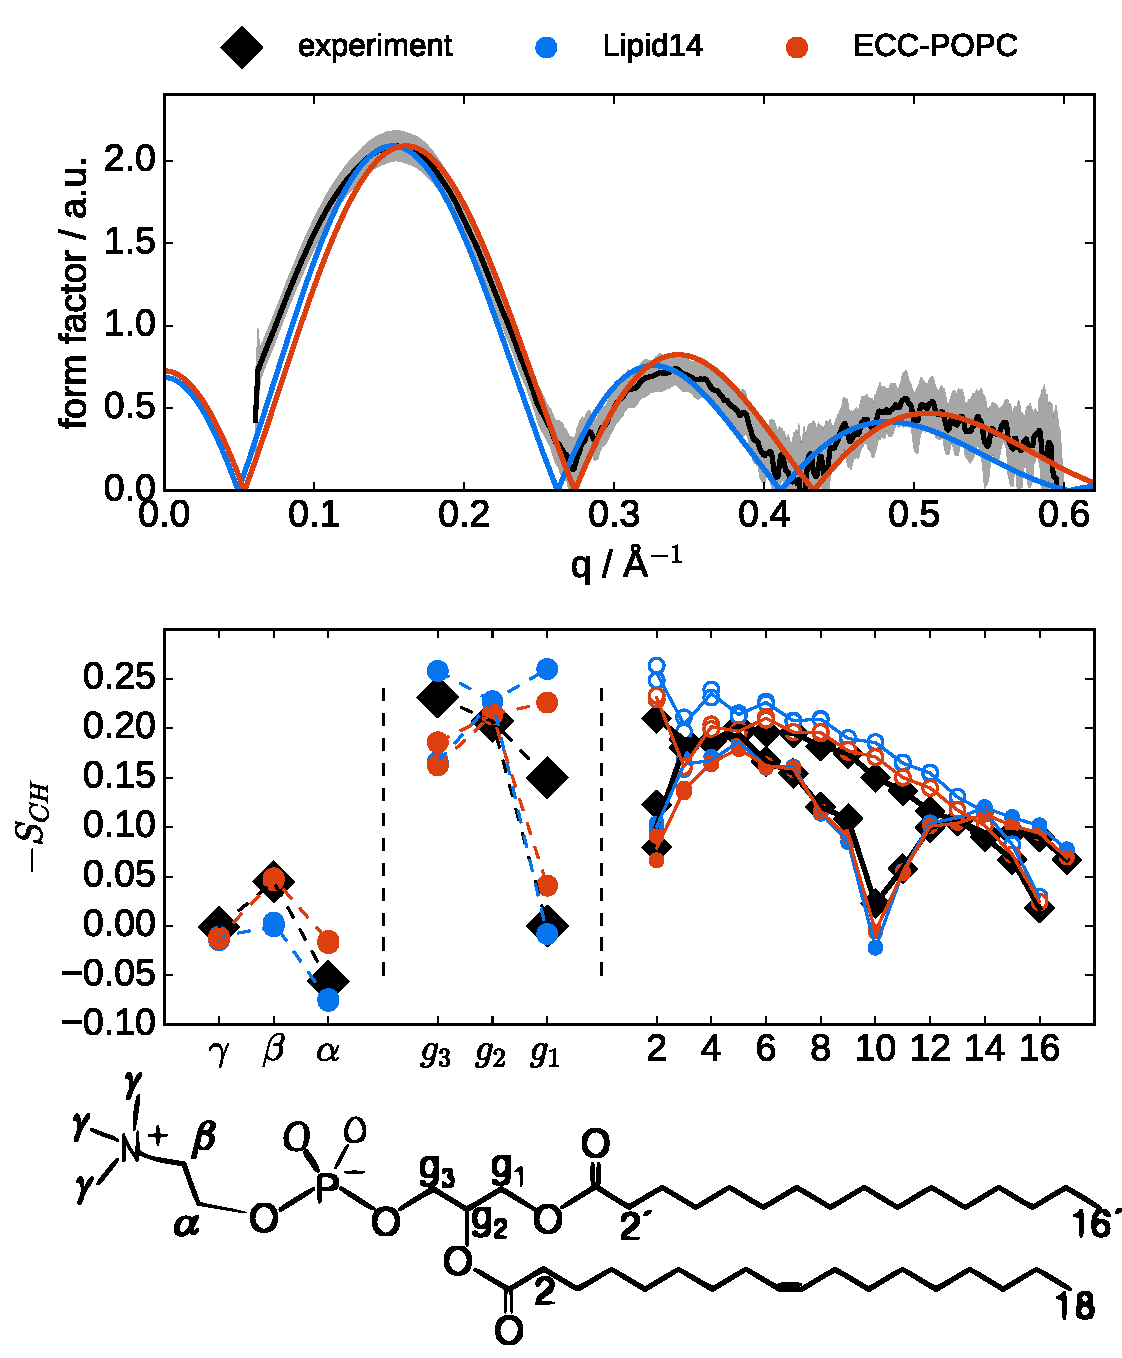
\includegraphics[width=\figwidth]{../img/ecc_popc/Order-parameters_form-factors_exp-L14-ECCL17_q80_sig89_POPC-struct.pdf} 
  \caption{ \label{fig:simVSexpNOions} 
    Top: X-ray scattering form factors from simulations with the Lipid14 \citep{dickson14} and 
    the ECC-POPC \citep{melcr18} models compared with experiments~\citep{kucerka11} at 303~K. 
    Middle: Order parameters of POPC head group, glycerol backbone and acyl chains  
    from simulations with the Lipid14 and the ECC-POPC models 
    compared with experiments \citep{ferreira13} at 300~K. 
    The size of the markers for the head group order parameters correspond to 
    the error estimate $\pm 0.02$ for experiments \citep{botan15,ollila16}, 
    while the error estimate for simulations is $\pm 0.005$
    (Bayesian estimate of 95\% confidence interval \citep{scipy}).
    The size of the points for acyl chains are decreased by a factor of 3 to improve the clarity of the plot.
    Open/closed symbols are used for palmitoyl/oleoyl chains of POPC. 
    Bottom: The chemical structure of POPC and the labeling of the carbon segments. 
  }  
\end{figure} 







Ion binding in lipid bilayers can be experimentally quantified
by measuring the changes of the head group order parameters in lipids.
In the case of the head group order parameters $\alpha$ and $\beta$ in phosphatidylcholine
(see Fig.~\ref{fig:simVSexpNOions} for the definition of the order parameters)
such changes are known under the term ''electrometer concept'' \citep{seelig87,catte16, ollila16}. 
It is experimentally observed that the C-H bond
order parameters of $\alpha$ and $\beta$ carbons in a PC lipid head group
are proportional to the amount of charge, positive or negative, bound per lipid~\citep{seelig87}.
The change of the order parameters measured with varying concentrations of aqueous ions 
can be then related to the amount of bound ions.


In our publications \citep{catte16, nmrlipids_proj4},
we have shown that such order parameters can be accurately determined also from MD simulations
and their changes correlate with the amount of bound charge in phospholipid bilayers, 
despite the inaccuracies in their actual structures without salts \citep{botan15}. 
It was found, however, that
none of the force fields examined in those works 
provided a sufficient accuracy for interpreting 
the experimentally measured structural changes induced by salt concentrations
and cation-lipid stoichiometries. 


A major improvement over currently available non-polarizable force fields
was achieved by developing new models of phospholipids, 
the so called ECC-lipids.
We developed models of POPC, POPE and POPS lipids,
which account for electronic polarization through electronic continuum correction (ECC), 
and which yield accurate response of the head group order parameters to various monovalent and divalent cations. \citep{melcr18}
In short, 
ECC is an implicit model of electronic polarizability,
which can be straightforwardly implemented into current force fields 
by scaling charges
without any extra computational costs compared to standard fixed-charge simulations. 
Our new model, ECC-lipids,
provides a proof of concept of the applicability of ECC
to charged as well as neutral molecules. 

We compared X-ray scattering form factors and NMR order parameters of bilayers
in pure water without any ions (or only counter ions)
from simulations and experiments
as the first step in the assessment of the quality of the model. 
The experimental X-ray scattering form factors 
of a bilayer are well reproduced for all lipids employing the presented ECC-lipids model 
(see Fig.~\ref{fig:simVSexpNOions}). 
The head group order parameters $\alpha$ and $\beta$ are highly relevant for this work,
as they are being used in the lipid electrometer concept. 
For POPC in pure water, the order parameter $\beta$ agrees well with the experiment, 
while the order parameter $\alpha$ is somewhat lower. 



%\begin{figure}[tbp!] 
%  \centering 
%  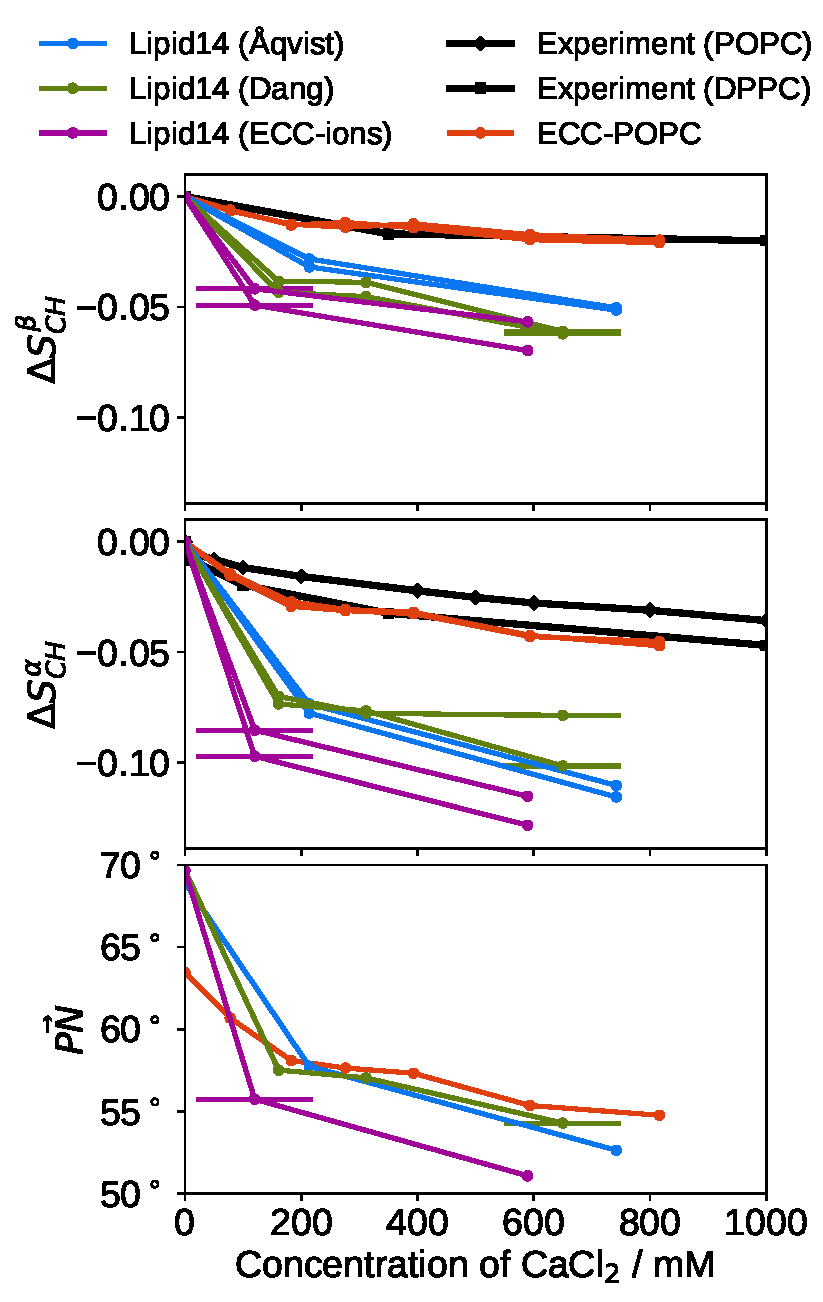
\includegraphics[width=\figwidth]{../img/ecc_popc/OrdPars-A-B-PNvec_L14-ECC-lipids_CaCl.pdf}
%  \caption{\label{fig:delta_ordPar_CaCl} 
%    Changes of the head group order parameters and P-N vector orientation of a POPC bilayer  
%    as a function of the CaCl$_2$ concentration in bulk ($C_{ion}$) 
%    from simulations at 313 K together with experimental data  
%    (DPPC (323\,K) \citep{akutsu81} and POPC (313\,K) \citep{altenbach84}).  
%    The error estimate for bulk concentrations is approximately 10\,mM. 
%    The order of magnitude larger error in the
%    simulation with Lipid14 and ECC-ions is due to unconverged bulk densities limited by the simulation box.  
%    Simulation data with Lipid14 and Åqvist ion parameters at 298~K are taken directly from 
%    Refs.~\citep{lipid14POPC0mMNaClfiles,lipid14POPC350mMCaClfiles,lipid14POPC350mMCaClfilesNC}. 
%  } 
%\end{figure} 


\begin{figure}[tb] 
  \centering 
  \subfloat[POPC bilayer]{\label{fig:delta_ordPar_CaCl} 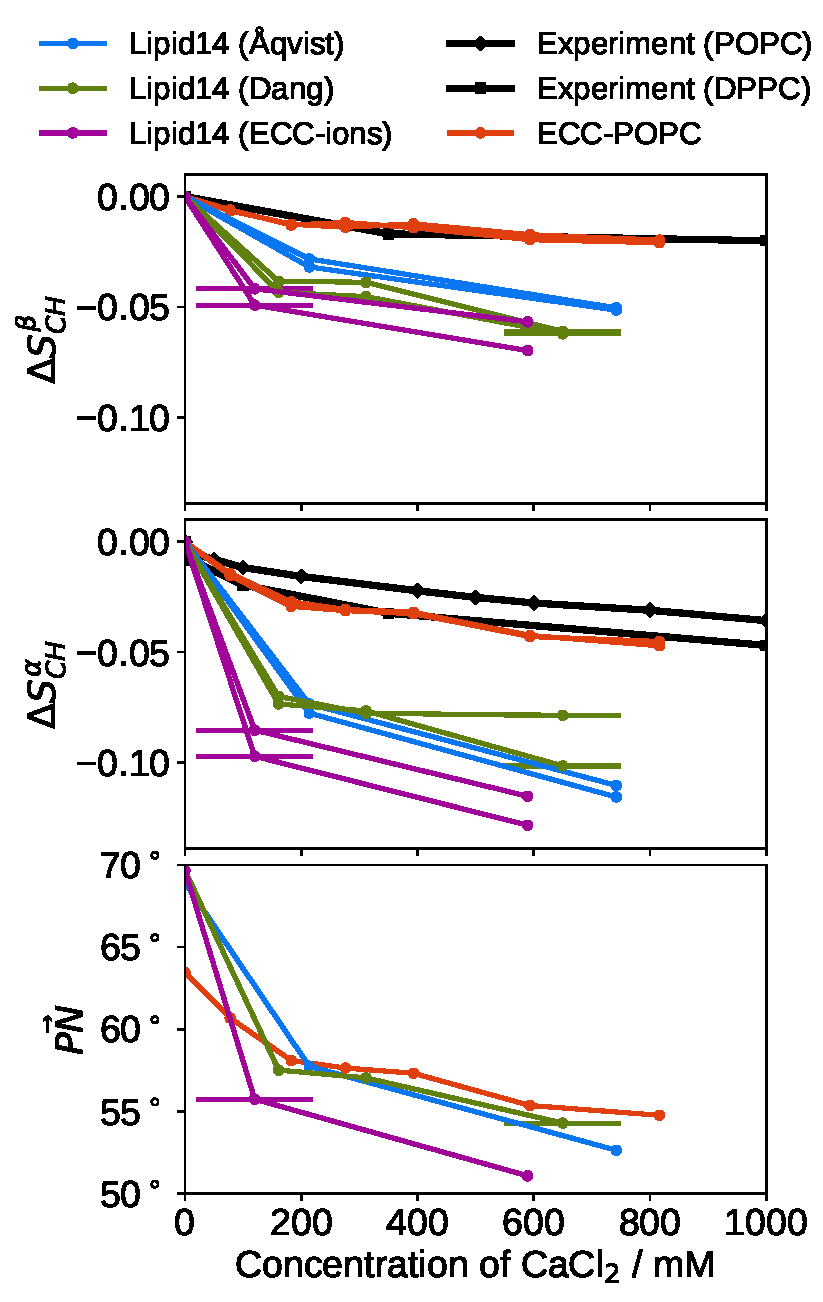
\includegraphics[width=\figwidthsmalltriple]{../img/ecc_popc/OrdPars-A-B-PNvec_L14-ECC-lipids_CaCl.pdf} }
  \subfloat[PC:PS (5:1) bilayer]{\label{fig:delta_ordPar_CaCl_PCPS} 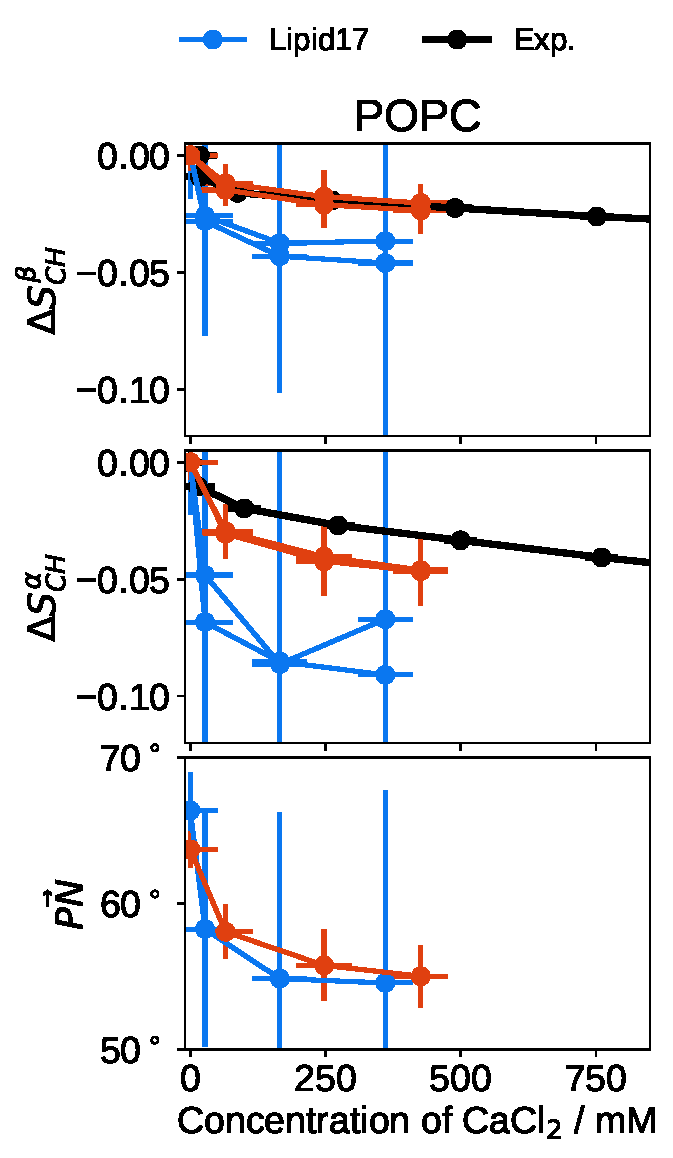
\includegraphics[width=\figwidthsmalltriple]{../img/ecc_pops/order_parameters_changes_ecc-lip_L14_A-B-PN-COO_POPC_cacl.pdf} }
  \subfloat[PC:PS (5:1) bilayer]{ 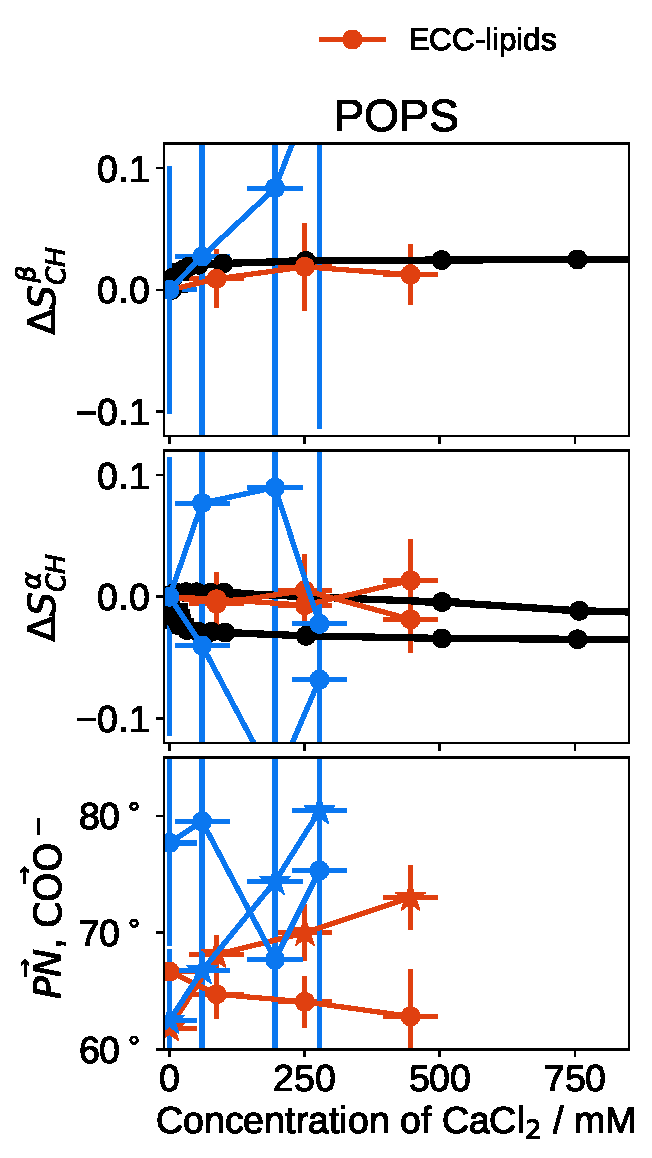
\includegraphics[width=\figwidthsmalltriple]{../img/ecc_pops/order_parameters_changes_ecc-lip_L14_A-B-PN-COO_POPS_cacl.pdf} }
  \caption{ 
    Changes of the head group order parameters $\alpha$, $\beta$ and the orientations of the carboxylate group and the P-N vector  
    of POPC (left, middle) and POPS (right) phospholipids in phospholipid bilayers as a function of \ce{CaCl2} concentration 
    in bulk ($C_{ion}$) from simulations with different force fields and experiments 
    (DPPC (323\,K) \citep{akutsu81} and POPC (313\,K) \citep{altenbach84}, PC:PS \citep{roux90}).  
    The orientation of the \ce{COO^-} group is defined as 
    the connector from the $\beta$ carbon to the carbon in \ce{COO^-} (stars, bottom right). 
  } 
\end{figure} 

 



%%% Sum up what is to be presented briefly

The changes of the head group order parameters $S^\alpha$ and $S^\beta$ from simulations and experiments 
are shown in Fig.~\ref{fig:delta_ordPar_CaCl} for a neutral POPC bilayer, 
and in Fig.~\ref{fig:delta_ordPar_CaCl_PCPS} for a negatively charged bilayer with the composition 5\,PC:1\,PS. 
For a direct comparison and a connection to our works \citep{catte16, nmrlipids_proj4},
we show simulation results from ECC-lipids and also from Lipid17 \citep{lipid17-future}. 
This also highlights the improvements in ECC-lipids over Lipid17 arising from the electronic polarization. 
%Although Lipid17 already belongs to the top-performing models in terms of the responses of the head group order parameters in those studies,  
%including electronic polarizability to form ECC-lipids improves the results even further.
The effect is probably the most striking for POPS, 
for which also the structure of a pure POPS bilayer with only counterions is dramatically improved with the augmentation. 


%%% Discuss the changes of OPs and vectors from neutral and neg. membranes
%While the changes induced by \ce{CaCl2} are \emph{qualitatively} correct for Lipid14/17, 
Increasing concentrations of \ce{CaCl2} induce a systematic decrease of the order parameters $S^\alpha$ and $S^\beta$ in POPC. 
Although the total magnitude of the response of the PC head group order parameters 
is only slightly higher in the negatively charged bilayers than in the neutral bilayers, 
the shape of the changes in the latter shows a steeper onset at low concentrations. 
This is apparently due to the presence of POPS, 
which has a higher affinity to \ce{Ca^{2+}} compared to POPC. 
ECC-lipids is the first model,
which achieves a \emph{quantitative} agreement with the changes induced by \ce{CaCl2} in experiments. 




\begin{figure}[tb] 
  \centering 
  %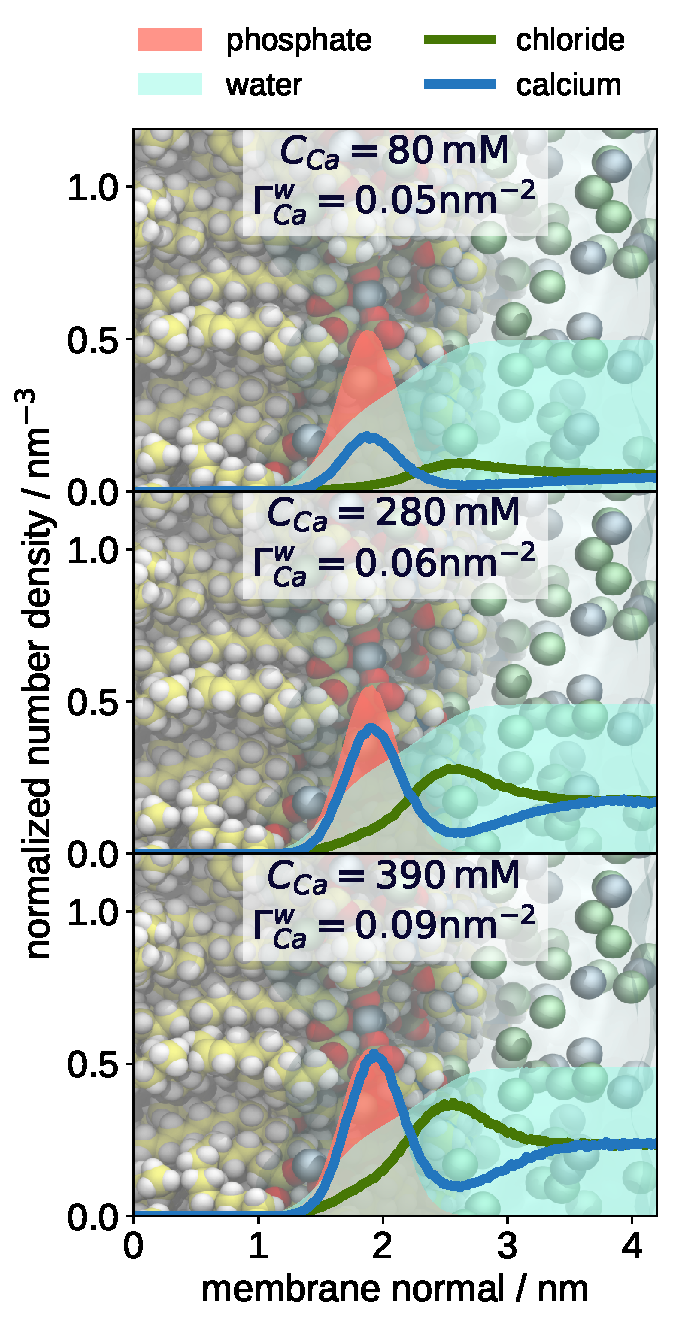
\includegraphics[width=\figwidth]{../img/ecc_popc/density_profiles_ca_cl_wat_phos_concentrations-compar.pdf} 
  \subfloat[POPC]{\label{fig:cacl-dens} 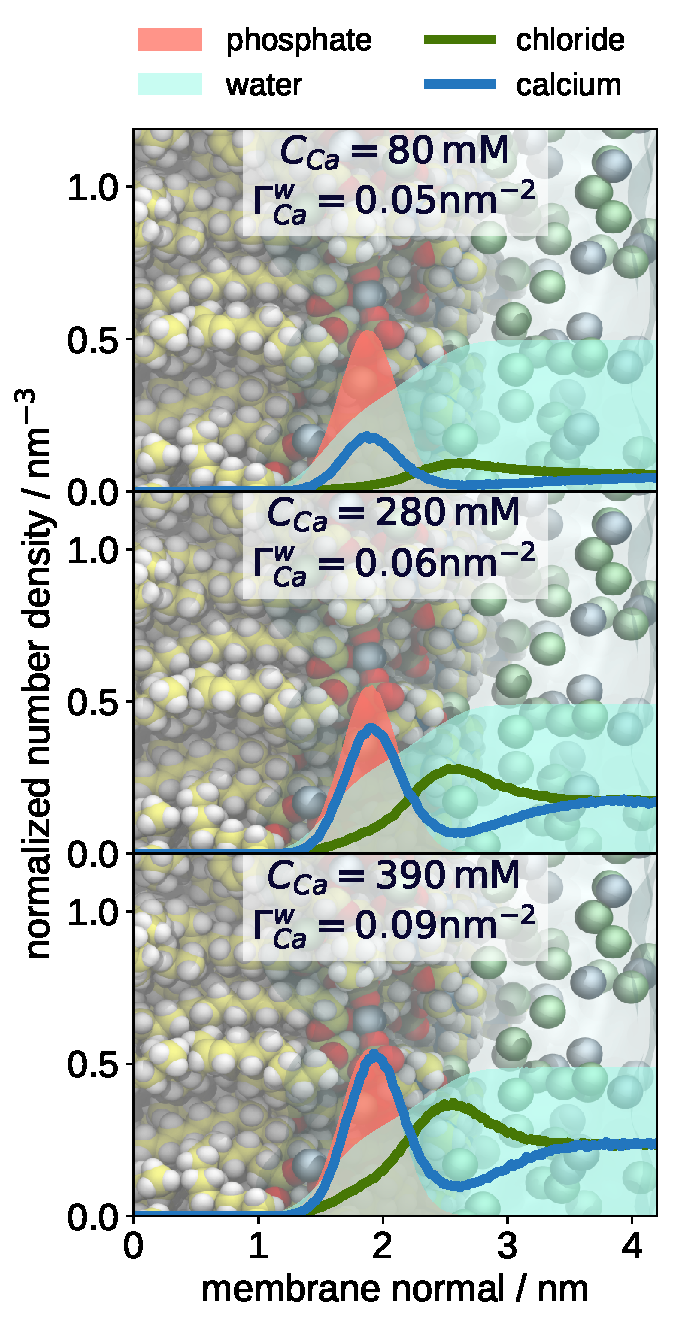
\includegraphics[width=\figwidthsmall]{../img/ecc_popc/density_profiles_ca_cl_wat_phos_concentrations-compar.pdf} }
  \subfloat[POPC:POPS (5:1)]{ \label{fig:cacl-dens_PCPS} 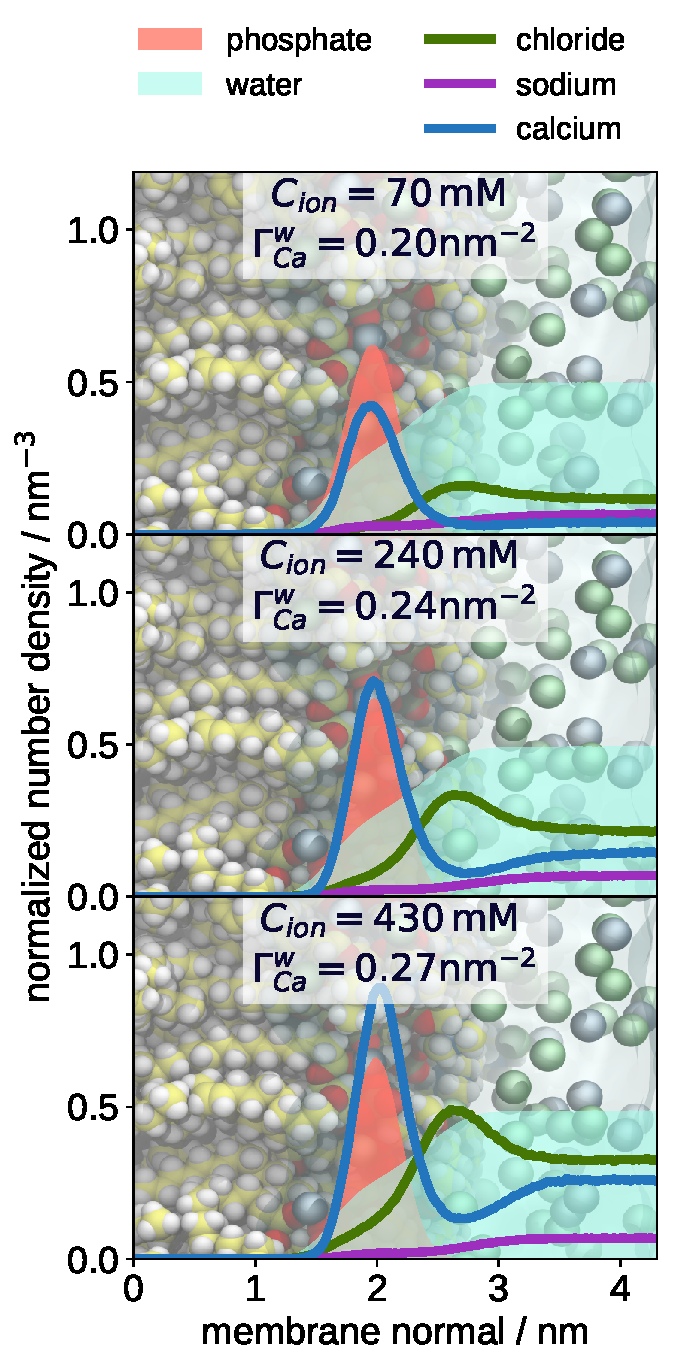
\includegraphics[width=\figwidthsmall]{../img/ecc_pops/density_profiles_ca_na_cl_wat_phos_models-compar_1-3_CaCl2-series.pdf} }
  \caption{ 
    Number density profiles of \ce{Ca^{2+}} and \ce{Cl^-} along the normal of the phospholipid bilayers starting at the centre 
    for different concentrations of \ce{CaCl2} from simulations with ECC-lipids. 
    In order to visualize the density profiles with a scale comparable to the profile of \ce{Ca^{2+}},  
    the density profiles of~\ce{Cl^-} ions are divided by 2, and 
    the density profiles of phosphate groups and water are divided by 5 and 200, respectively.  
    } 
\end{figure} 


%\begin{figure}[htbp!] 
%  \centering 
%  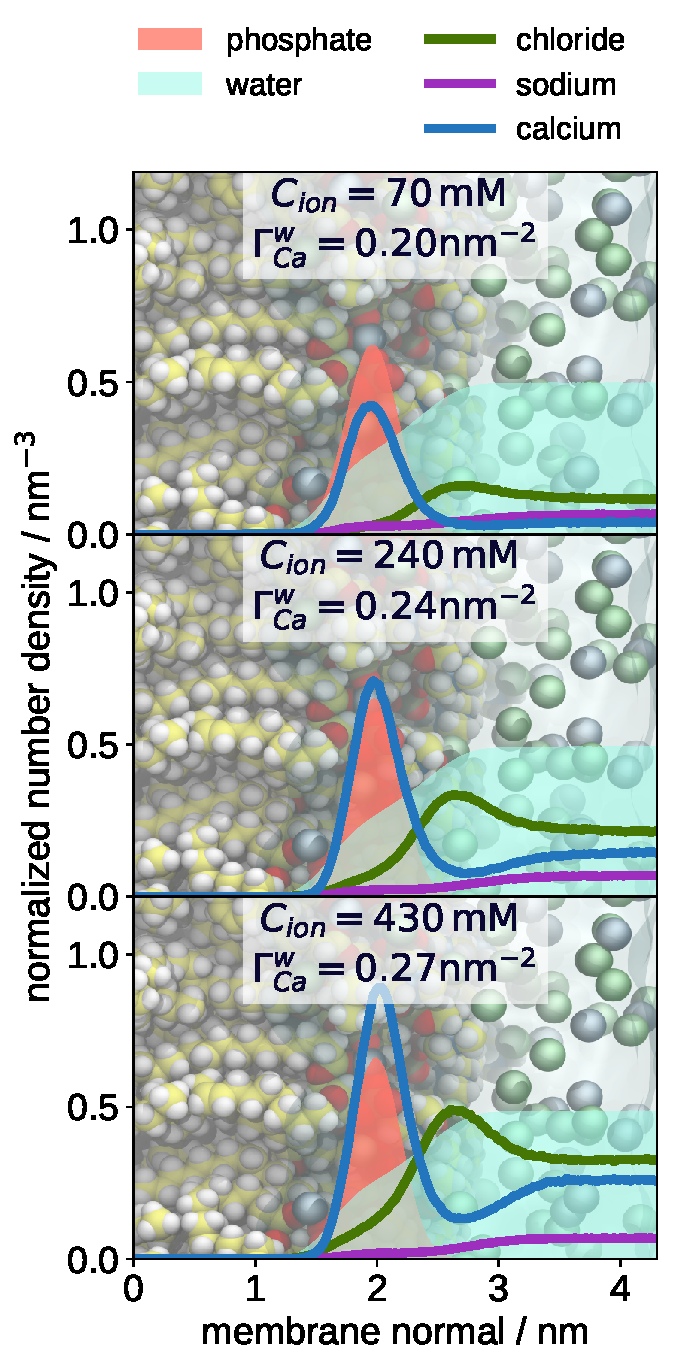
\includegraphics[width=\figwidth]{../img/ecc_pops/density_profiles_ca_na_cl_wat_phos_models-compar_1-3_CaCl2-series.pdf}
%  \caption{\label{fig:cacl-dens_PCPS} 
%    Number density profiles of \ce{Ca^{2+}}, \ce{Na^{+}} and \ce{Cl^-} along the normal of the membrane starting at the centre
%    for the negatively charged membrane with the composition 5\,PC:1\,PS
%    at various bulk concentrations of \ce{CaCl2} from simulations with ECC-lipids. 
%    All profiles contain \ce{Na^+} counterions and an additional concentration of \ce{CaCl2}. 
%    In order to visualize the density profiles with a scale comparable to the profile of \ce{Ca^{2+}},  
%    the density profiles of~\ce{Cl^-} ions are divided by 2, and 
%    the density profiles of phosphate groups and water are divided by 5 and 200, respectively.  
%    } 
%\end{figure} 
 





%%% Present the density profiles (different concentrations for both POPC and mixed)
The increase in the amount of bound calcium cations from pure POPC to the mixed negatively charged bilayer containing POPS
is well demonstrated using the relative surface excess, $\Gamma ^w _{Ca}$.
Distributions of \ce{Ca^{2+}}, \ce{Na^+} counterions and also \ce{Cl^-} 
are plotted in Fig.~\ref{fig:cacl-dens} for the neutral POPC bilayer, 
and in Fig.~\ref{fig:cacl-dens_PCPS} for the negatively charged bilayer. 
The increasing concentration of \ce{CaCl2} and, hence, a higher amount of bound \ce{Ca^{2+}}
attracts \ce{Cl^-} anions to the bilayer 
as can be seen from its growing density at the interface. 
%%% discuss the table with Gammas and follow up with molecular details, where do cations bind? Support with the spatial density figure
The density profiles of ions suggest that
the dominant contribution to the binding of \ce{Ca^{2+}} to phospholipid bilayers
comes from the interactions with the phosphate groups in both POPC and POPS. 
%The population analysis also suggests 
%that the calcium cations prefer to reside in the phosphate region of the membrane. 
%Such a finding is further validated with a more detailed analysis using Markov state modeling (MSM) \citep{Pande_MSM_paper} \todoi{Add papers reviewing MSM, e.g. recent Pande's paper.}. 
%The set of states of a calcium cation 
%encompassed all possible combinations of up to three surrounding lipids. 
%In the case of PC, we used only the phosphate moitety, which forms the dominant contribution for calcium binding.
%For PS we also distinguished configurations in which calcium interacts with the carboxylate moiety. 
%All possible combinations of such states were used to build a Markov model at a lag time $25\,\mathrm{ns}$ using pyEMMA code by \citet{pyemma} \todoi{add citation for pyemma}. 
%The resulting MSM was validated using Chapman-Kolmogorov test \citep{FrankNoe_papers_MSM} \todoi{Add citation for Noe's papers on MSM, especially Chapman Kolmogorov test.}. 
%The stationary distribution of the states reveals a strong preference of the calcium cations to reside in the phosphate region of the mixed PC-PS membrane. 
%When interacting with PS, configurations with the phosphate moiety from either PC or PS dominate the population.
%Moreover, states containing interactions with the carboxylate group in PS 
%bear higher probability when interacting also with the phosphate group of the same lipid or other lipids. 
This is also reflected in the shift of the mean orientation 
of the \ce{COO^-} group from $62^\circ$ to $73^\circ$ (420~mM \ce{CaCl2})
which was measured as the connector of the carbon atoms 
forming the bond between the group and the $\beta$-carbon of the phospholipid. 
The interactions of the carboxylate group in PS with calcium and other phosphate groups
shed light into the qualitatively different response of the head group order parameters $\alpha$ and $\beta$ in PS compared to PC 
(see Figs.~\ref{fig:delta_ordPar_CaCl} and~\ref{fig:delta_ordPar_CaCl_PCPS}). 
We find that the complex response of the head group order parameters of POPS 
is affected by the conformational changes of the carboxylate group,
which is attracted more towards the phosphate region, 
where the calcium cations dominantly bind. 
In line with the experimental work by \citet{browning80},
this is also very likely the reason, 
why the magnitude of the P-N vector change in POPS is diminished compared to POPC, 
which is not restrained by an additional cation binding group like \ce{COO^-} in POPS. 









%%%%%%%%%%%%%%%%%%%%%%%%%%%%%%%%%%%%%%%%%%%%%%%%%%
%%%%%%%%%%%%%%%%%%%%%%%%%%%%%%%%%%%%%%%%%%%%%%%%%%
%%%%%%%%%%%%%%%%%%%%%%%%%%%%%%%%%%%%%%%%%%%%%%%%%%

\section*{Modeling of transmembrane potential}
\addcontentsline{toc}{section}{Modeling of transmembrane potential}

The intracellular environment of cells contains a weak electrolytic solution of \ce{KCl}, 
while there is a similarly weak solution of \ce{NaCl} on the extracellular side. 
The concentrations of these salts, usually around 150\,mM, 
are regulated and maintained out of equilibrium through specific channels and pumps 
to provide cellular functions and general homeostasis conditions \citep{Bezanilla2008, Knudsen_book2002}. 
The unequal distribution of ions on either side of the membrane
gives rise to a transmembrane potential. 
For instance, the concerted action of voltage-gated ion channels and pumps in neurons 
modulates their transmembrane potential
providing a fast signal transduction through the axons \citep{Knudsen_book2002, Storace2015, Sung2015}. 
A common magnitude of the transmembrane potential in cells is in the range of 10--100~mV. 

The transmembrane potential in simulations can be modeled by several methods. \citep{Tieleman2001,Sin2015, Roux1997, sachs04_potential}.
In particular, 
there are two approaches for the modeling of 
the membrane potential in atomistic molecular dynamics simulations --
 the constant electric field method \citep{Roux1997,Roux2008,gumbart_constant_2012}, 
and
 the ion-imbalance method \citep{sachs04_potential,Delemotte2008}. 
Both of these methods have been successfully used to study membrane electroporation or voltage-sensitive proteins \citep{Vargas2012, bockmann_kinetics_2008, gumbart_constant_2012, kutzner_computational_2011, casciola_molecular_2014}. 
These two practically independent developments were compared and connected together in our work \citep{melcr16},
where we prove them to be equivalent models of the transmembrane potential yielding indistinguishable results, 
at least for electrolytes formed by the same monovalent ions on both sides of the membrane. 
We used simulations 
in which we simultaneously applied both methods
with the same magnitude but opposite polarity 
yielding zero transmembrane voltage in total 
to highlight possible artifacts. 
The comparison in Fig.~\ref{fig:potentialKCl} shows 
that such a setup is indistinguishable 
from simulations without voltage within the achievable accuracy. 
The electric field induced by the voltage 
exists exclusively in the hydrophobic region of the membrane,
where it has an almost constant strength. 
This finding provides clues to understanding the evolutionary design of voltage-gated proteins. \citep{Vargas2012} 
Moreover,
the structure of the bilayer is preserved even at high voltages at the time scales of our simulations,
unlike that of water at the interface with the hydrophobic core of the bilayer
underlining its importance in electroporation. \citep{bu2017mechanics}

\begin{figure}[bt!]
\begin{center}
\includegraphics[width = \figwidthfull]{../img/pot+field+chargedens_6plot_KCl-page001.png}
 \caption{The transmembrane potential (A,B), the electric field intensity (C,D), and the charge density (E,F) profiles for simulations of a POPC bilayer with 150\,mM concentration of \ce{KCl}. 
ZERO stands for simulations without any applied voltage,
IIMB stands for the ion imbalance method,
CEF  stands for the constant electric field method,
and FxI denotes the special setup, in which the two methods are applied simultaneously. 
The gray area shows the standard error. 
The voltage drop across the membrane is $499\,$mV for IIMB and $486\,$mV for CEF with the error of about $7\,$mV.  
}
\label{fig:potentialKCl}
\end{center}
\end{figure}











%%% Bibliography
%%% Bibliography (literature used as a source)
%%%
%%% We employ bibTeX to construct the bibliography. It processes
%%% citations in the text (e.g., the \cite{...} macro) and looks up
%%% relevant entries in the bibliography.bib file.
%%%
%%% The \bibliographystyle command selects, which style will be used
%%% for references from the text. The argument in curly brackets is
%%% the name of the corresponding style file (*.bst). Both styles
%%% mentioned in this template are included in LaTeX distributions.

\bibliographystyle{plainnat}    %% Author (year)
% \bibliographystyle{unsrt}     %% [number]

\renewcommand{\bibname}{Bibliography}

%%% Generate the bibliography. Beware that if you cited no works,
%%% the empty list will be omitted completely.

\bibliography{bibliography}

%%% If case you prefer to write the bibliography manually (without bibTeX),
%%% you can use the following. Please follow the ISO 690 standard and
%%% citation conventions of your field of research.

% \begin{thebibliography}{99}
%
% \bibitem{lamport94}
%   {\sc Lamport,} Leslie.
%   \emph{\LaTeX: A Document Preparation System}.
%   2nd edition.
%   Massachusetts: Addison Wesley, 1994.
%   ISBN 0-201-52983-1.
%
% \end{thebibliography}



%%% Doctoral theses must contain a list of author's publications
\chapwithtoc{List of publications}

%%% Attachments to the doctoral thesis, if any. Each attachment must be
%%% referred to at least once from the text of the thesis. Attachments
%%% are numbered.
%%%
%%% The printed version should preferably contain attachments, which can be
%%% read (additional tables and charts, supplementary text, examples of
%%% program output, etc.). The electronic version is more suited for attachments
%%% which will likely be used in an electronic form rather than read (program
%%% source code, data files, interactive charts, etc.). Electronic attachments
%%% should be uploaded to SIS and optionally also included in the thesis on a~CD/DVD.
%%% Allowed file formats are specified in provision of the rector no. 72/2017.
%\chapter{Attachments}

\begin{itemize}
% paper Transmembrane potential modeling, JCTC 2016
\item[I] 
Transmembrane Potential Modeling: Comparison between Methods of Constant Electric
Field and Ion Imbalance. 
Journal of Chemical Theory and Computation, 12(5), (2016). 
\textbf{Josef Melcr}, Daniel Bonhenry, Štěpán Timr, and Pavel Jungwirth. 

% paper NMRLipids II project -- lipid-ion interaction PCCP 2016
\item[II] 
Molecular electrometer and binding of cations to phospholipid bilayers. 
Phys. Chem. Chem. Phys., (2016).
Andrea Catte, Mykhailo Girych, Matti Javanainen, Claire Loison, \textbf{Josef Melcr},
Markus S. Miettinen, Luca Monticelli, Jukka Maatta, Vasily S. Oganesyan,
O. H. Samuli Ollila, Joona Tynkkynen, and Sergey Vilov. 

\item[III]
Accurate Binding of Sodium and Calcium to a POPC Bilayer by Effective Inclusion of Electronic Polarization. (2018)
The Journal of Physical Chemistry B, 122(16), (2018).
\textbf{Josef Melcr}, Hector Martinez-Seara, Ricky Nencini, Jiří Kolafa, Pavel Jungwirth,
and O. H. Samuli Ollila. 

\item[IV]
Head group and glycerol backbone structures,
and cation binding in bilayers with PS lipids. Submitted (2018).
Amelie Bacle, Pavel Buslaev, Lukasz Cwiklik, Fernando Favela, Tiago Ferreira,
Patrick Fuchs, Ivan Gushchin, Matti Javanainen, Batuhan Kav, Jesper Madsen, 
\textbf{Josef Melcr}, Markus Miettinen, Ricky Nencini,  Chris Papadopoulos, Thomas Piggot 
and O. H. Samuli Ollila. 

\end{itemize}

\appendix

\openright
\end{document}
